%%%%%%%%%%%%%%%%%%%%%%%%%%%%%%%%%%%%%%%%%%%%%%%%%%%%%%%
\documentclass{article}
%%%%%%%%%%%%%%%%%%%%%%%%%%%%%%%%%%%%%%%%%%%%%%%%%%%%%%%
\usepackage[utf8]{vietnam}
%%%%%%%%%%%%%%%%%%%%%%%%%%%%%%%%%%%%%%%%%%%%%%%%%%%%%%%
\usepackage{graphicx}
%%%%%%%%%%%%%%%%%%%%%%%%%%%%%%%%%%%%%%%%%%%%%%%%%%%%%%%
\usepackage{hyperref}
%%%%%%%%%%%%%%%%%%%%%%%%%%%%%%%%%%%%%%%%%%%%%%%%%%%%%%%
\usepackage{xcolor}
\pagecolor[RGB]{40, 42, 54} % Đặt màu nền
\color[RGB]{18, 161, 24} % Đặt màu chữ
%%%%%%%%%%%%%%%%%%%%%%%%%%%%%%%%%%%%%%%%%%%%%%%%%%%%%%%
\usepackage{float} % Cố định hình ảnh [H]
%%%%%%%%%%%%%%%%%%%%%%%%%%%%%%%%%%%%%%%%%%%%%%%%%%%%%%%
\begin{document}
%%%%%%%%%%%%%%%%%%%%%%%%%%%%%%%%%%%%%%%%%%%%%%%%%%%%%%%
\tableofcontents
\newpage
%%%%%%%%%%%%%%%%%%%%%%%%%%%%%%%%%%%%%%%%%%%%%%%%%%%%%%%
\listoffigures
\newpage
%%%%%%%%%%%%%%%%%%%%%%%%%%%%%%%%%%%%%%%%%%%%%%%%%%%%%%%
\section{Tuần 3: Xây dựng dashboard}
%%%%%%%%%%%%%%%%%%%%%%%%%%%%%%%%%%%%%%%%%%%%%%%%%%%%%%%
\subsection{Bài 1}

\subsubsection{Thực hành tạo dashboard theo video}

\begin{figure}[H]
\centering
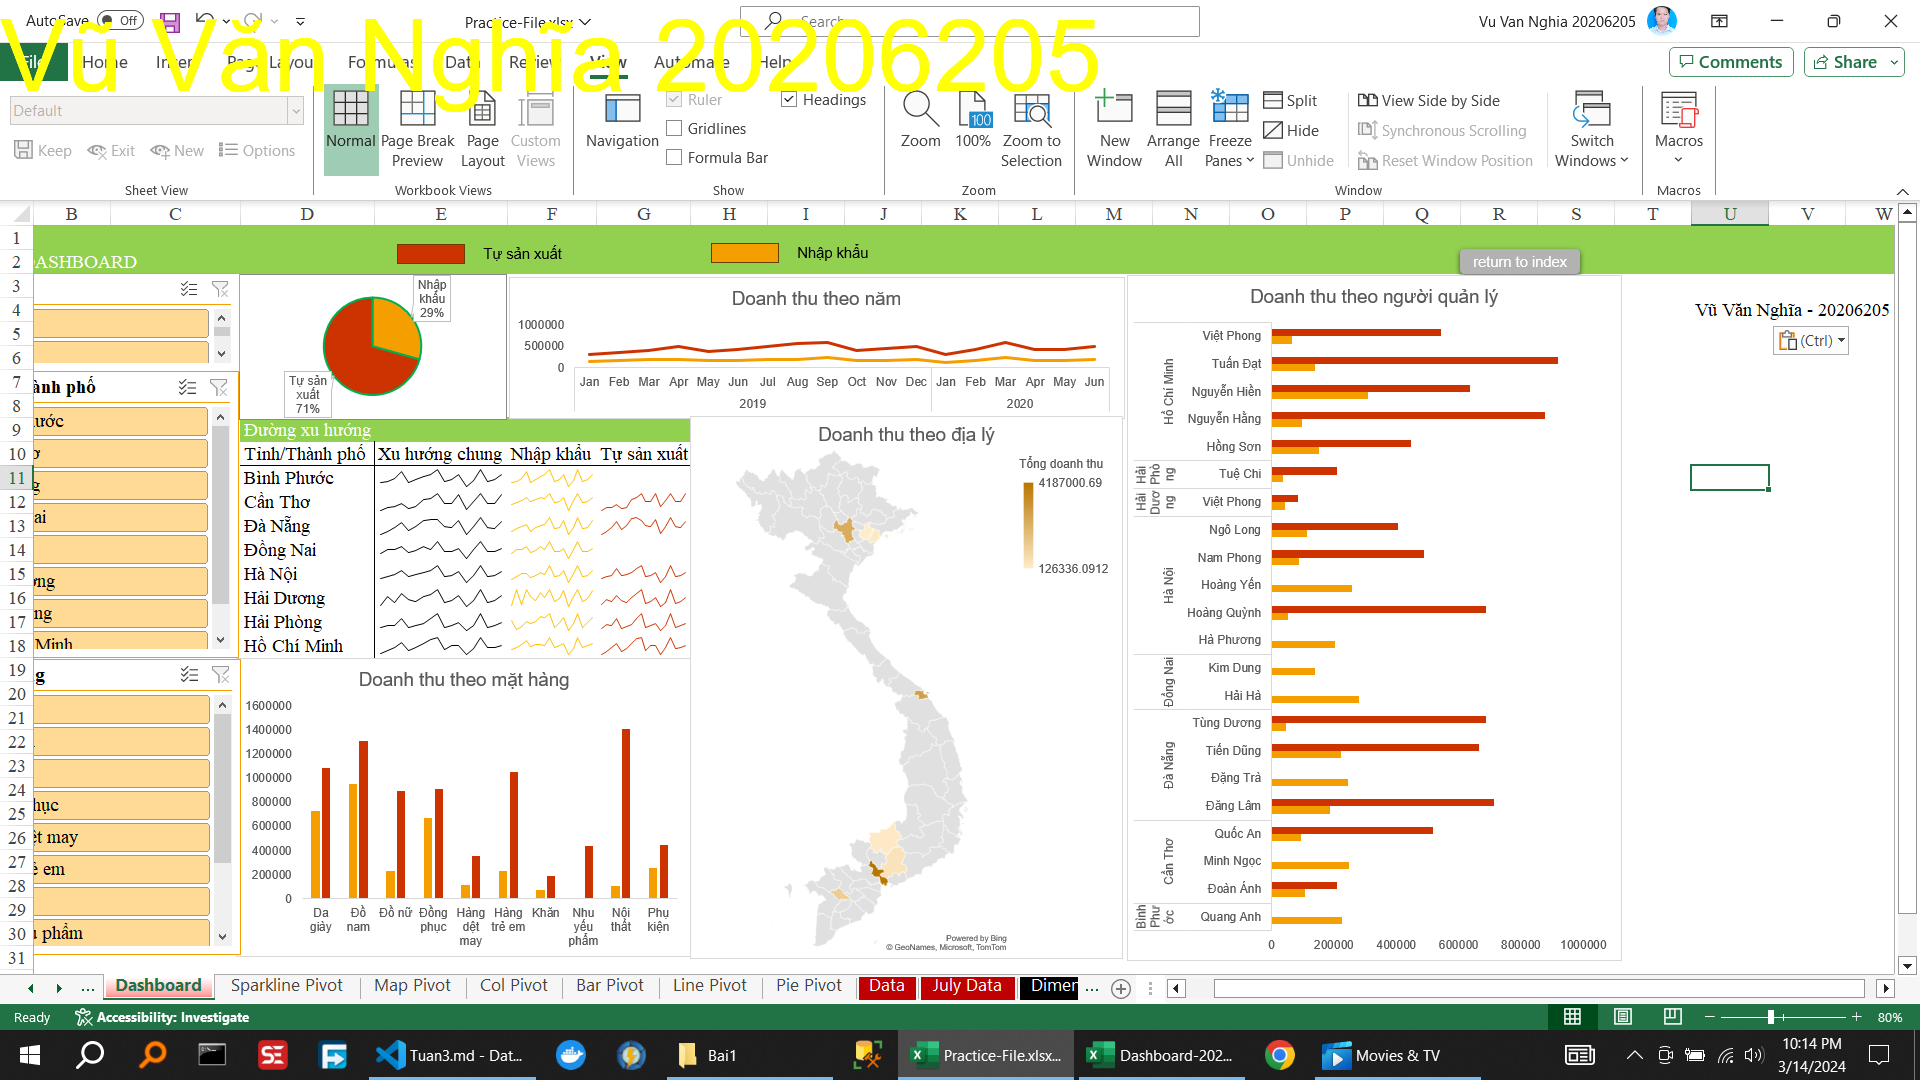
\includegraphics[scale = 0.15]{Bai1/ThucHanh/0.png}
\caption{Thực hành tạo dashboard theo video}
\end{figure}

\subsubsection{Thực hành phân tích dashboard}

\begin{itemize}
\item Đọc dashboard và  phân tích 
\begin{itemize}
\item Dashboard dùng để         mô tả  về doanh số bán hàng   cho thị trường Việt Nam.
\item Dashboard có các biểu đồ:
\begin{itemize}
\item Biểu đồ tròn: thể hiện tỷ lệ nhập khẩu và tự sản xuất.
\item Biểu đồ đường: thể hiện doanh thu theo năm.
\item Biểu đồ thanh: thể hiện doanh thu theo người quản lý.
\item Biểu đồ cột: thể hiện doanh thu theo mặt hàng.
\item Biểu đồ bản đồ: thể hiện doanh thu theo địa lý.
\end{itemize}
\end{itemize}
\item Xác định các chiều (DIM), các các yếu tố phân tích (FACT)

\begin{figure}[H]
\centering
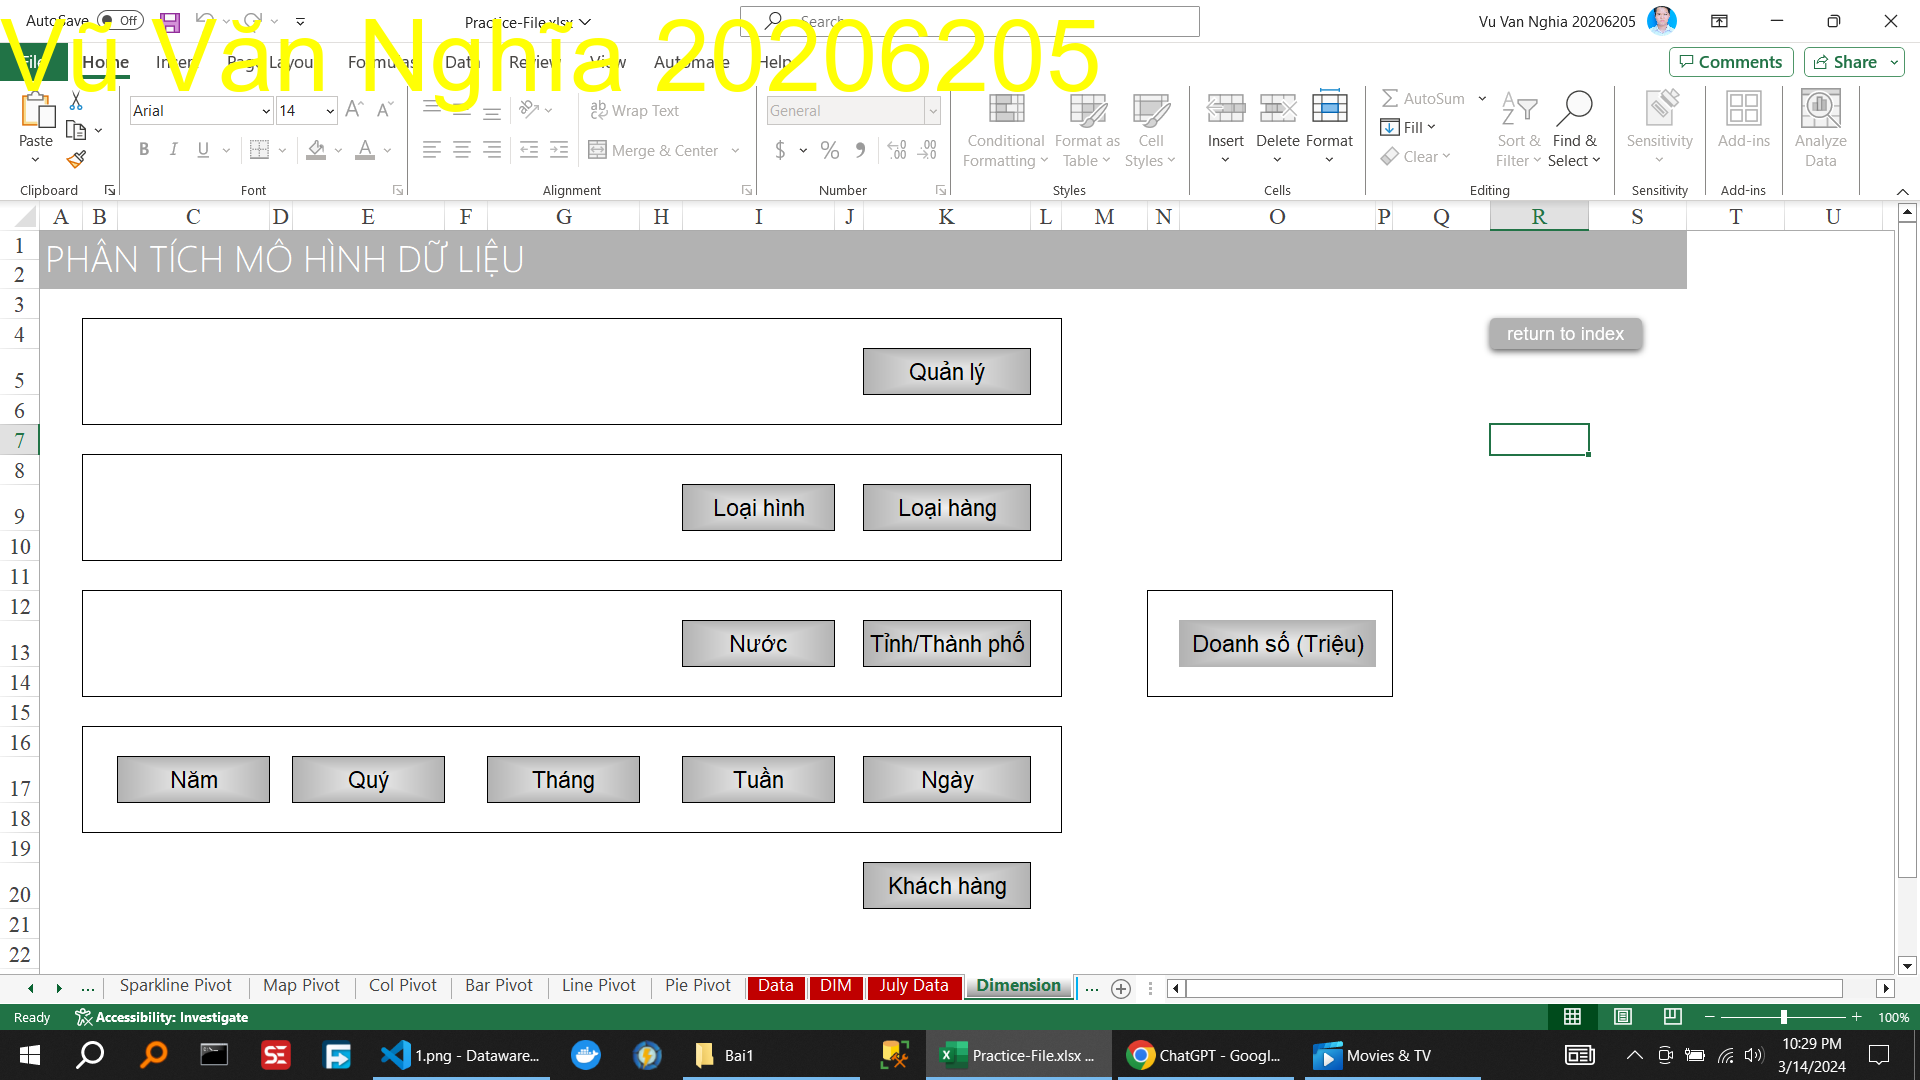
\includegraphics[scale = 0.15]{Bai1/ThucHanh/1.png}
\caption{Thực hành xác định các chiều (DIM), các các yếu tố phân tích (FACT)}
\end{figure}

\begin{itemize}
\item DIM: Thời gian, Năm, Loại hình Sản xuất, Tỉnh/Thành phố, Nước, Quản lý, Mặt hàng, Khách hàng.
\item FACT: Doanh số (Triệu).
\end{itemize}

\item Sử dụng công cụ Remove Duplicate để tạo ra con voi khái niệm các chiều.

\begin{figure}[H]
\centering
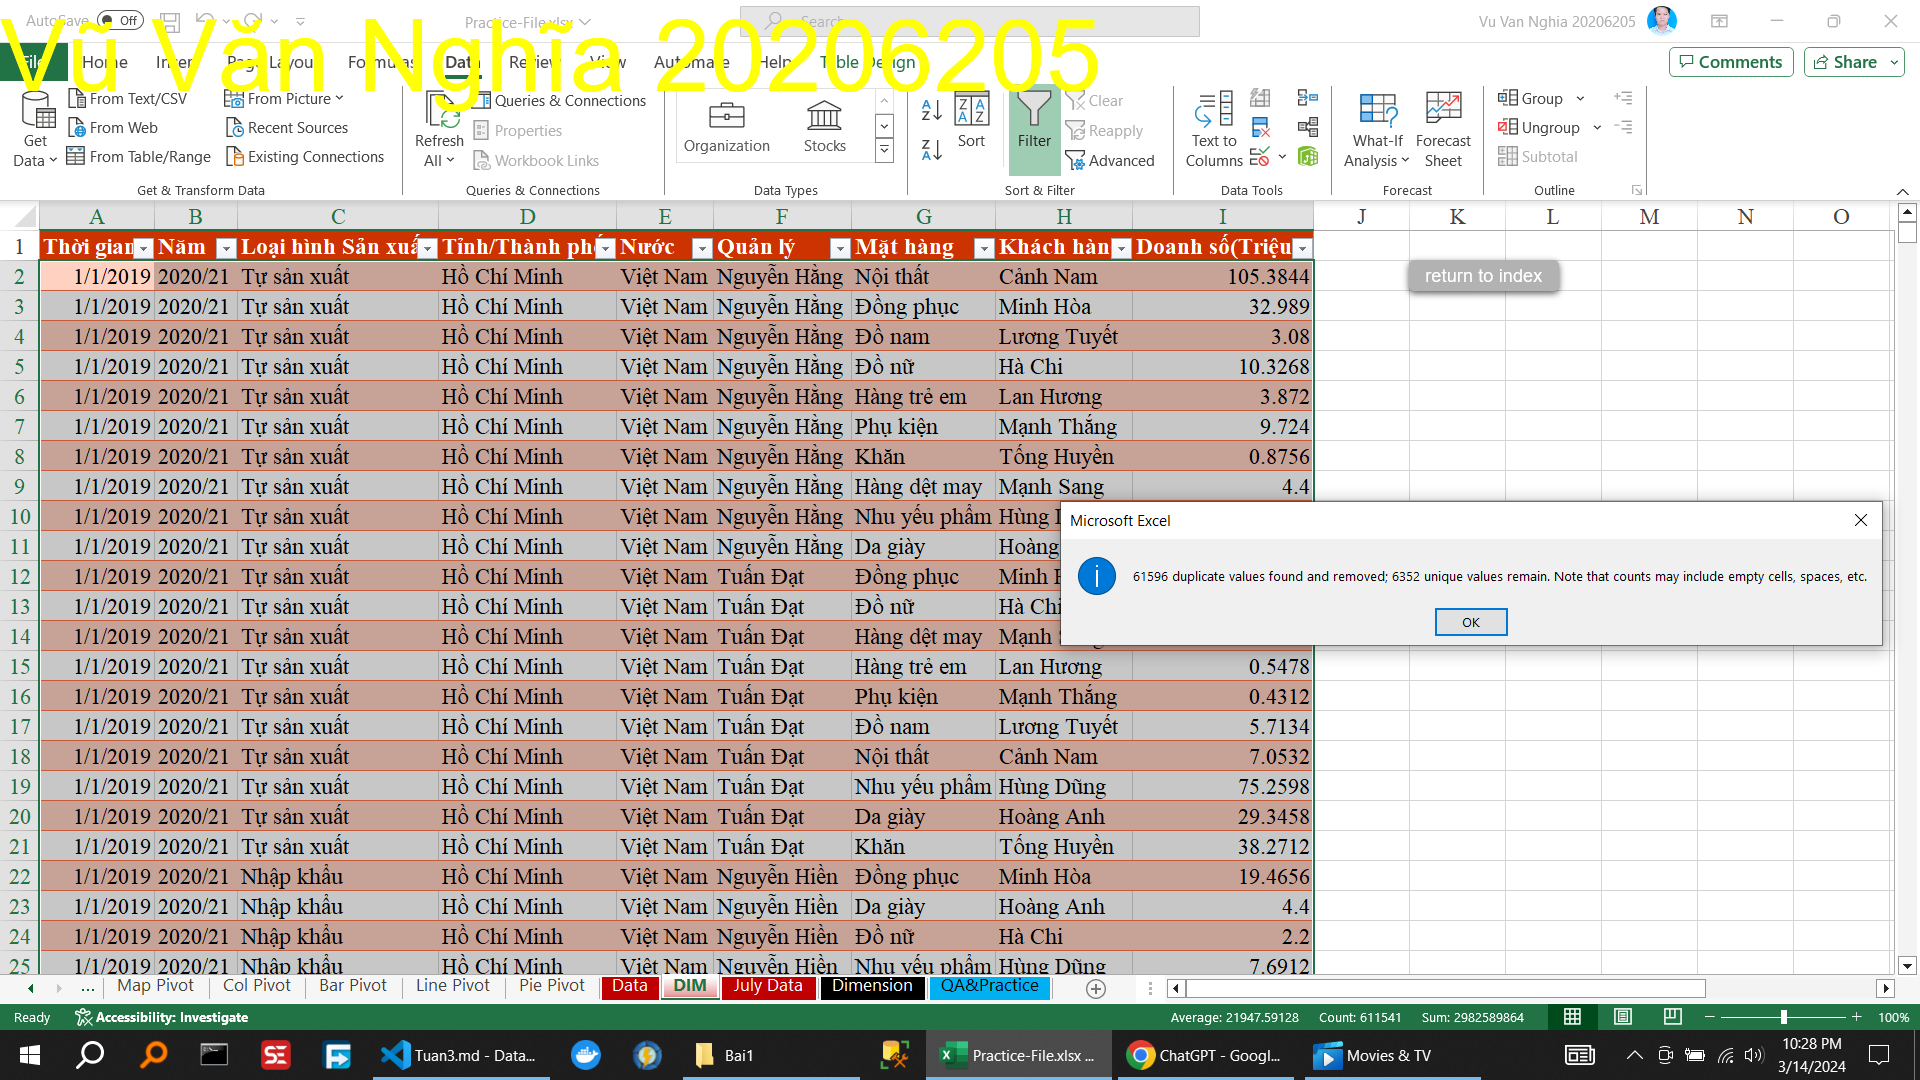
\includegraphics[scale = 0.15]{Bai1/ThucHanh/2.png}
\caption{Thực hành sử dụng công cụ Remove Duplicate để tạo ra con voi khái niệm các chiều}
\end{figure}

\end{itemize}

%%%%%%%%%%%%%%%%%%%%%%%%%%%%%%%%%%%%%%%%%%%%%%%%%%%%%%%
\subsection{Bài 2}

% \begin{figure}[H]
% \centering
% 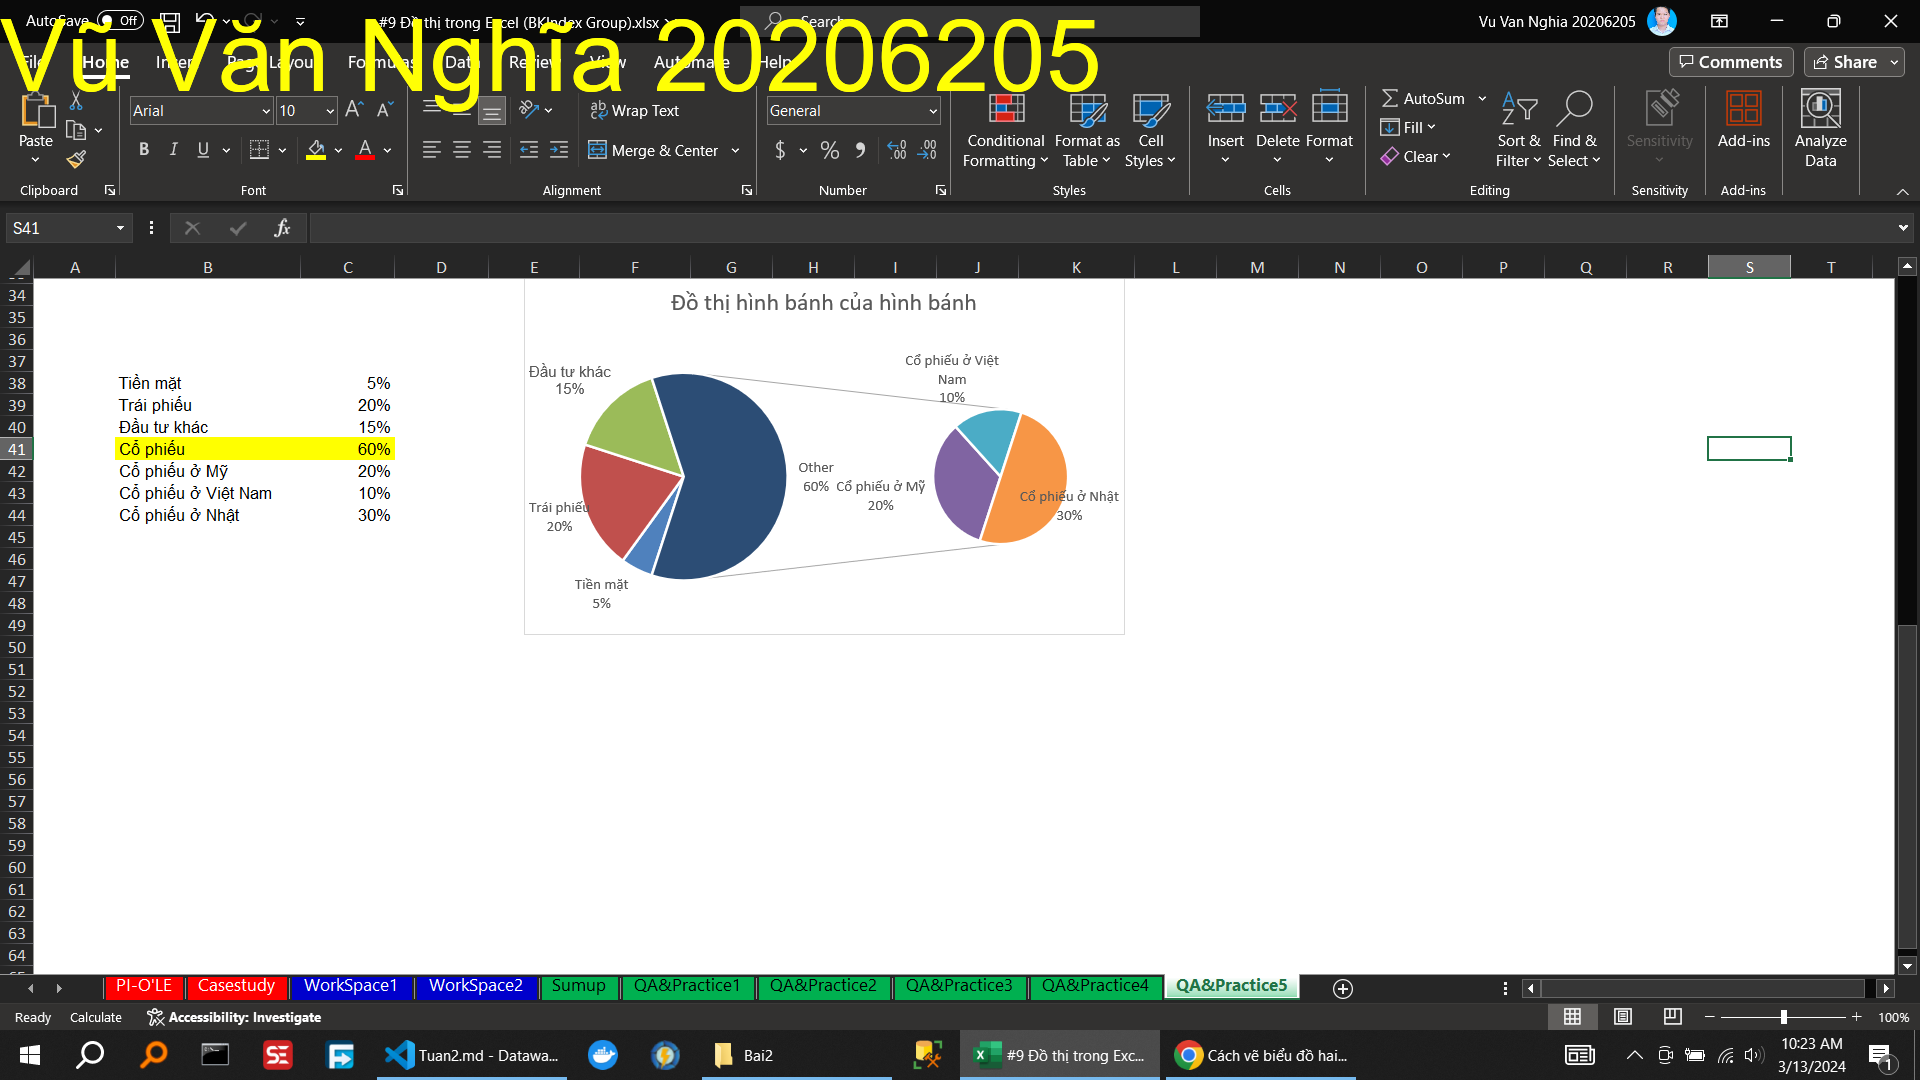
\includegraphics[scale = 0.15]{Bai2/ThucHanh/3.png}
% \caption{Thực hành vẽ đồ thị hình bánh của hình bánh}
% \end{figure}

%%%%%%%%%%%%%%%%%%%%%%%%%%%%%%%%%%%%%%%%%%%%%%%%%%%%%%%
\end{document}
%%%%%%%%%%%%%%%%%%%%%%%%%%%%%%%%%%%%%%%%%%%%%%%%%%%%%%%